\documentclass{cubeamer}
\usepackage[all,cmtip]{xy}
\newcommand{\mcU}{\mathcal{U}}
\newcommand{\mcO}{\mathcal{O}}
\newcommand{\mcI}{\mathcal{I}}
\newcommand{\mcL}{\mathcal{L}}
\newcommand{\mcS}{\mathcal{S}}
\newcommand{\hilbert}{{\sf H}}
\newcommand{\mcB}{\mathcal{B}}
\newcommand{\mcH}{\mathcal{H}}
\newcommand{\mcF}{\mathcal{F}}
\newcommand{\mcC}{\mathcal{C}}
\newcommand{\mcT}{\mathcal{T}}
\newcommand{\mcE}{\ensuremath{\mathcal{E}} }
\newcommand{\mcG}{\ensuremath{\mathcal{G}} }
\newcommand{\mcM}{\mathcal{M}}
\newcommand{\mcN}{\mathcal{N}}
\newcommand{\nnn}{\mathcal{N}}
\newcommand{\choi}{\ensuremath{\mcD} }
\newcommand{\mmm}{\mathcal{M}}
\newcommand{\sss}{\mathcal{S}}
\newcommand{\mcD}{\mathcal{D}}
\newcommand{\mcA}{\mathcal{A}}
\newcommand{\mcP}{\mathcal{P}}
\newcommand{\Complex}{\mathbb{C}} %Para escribir al espacio de hilbert complejo
\newcommand{\Id}{\mathds{1}}% Para escribir el op. indentidad con notación chida
\newcommand{\CG}[1]{\mcC\left[#1\right]}
\newcommand{\Fuzzy}[1]{\mcF\left[#1\right]}
\newcommand{\nota}[1]{{\color{red} [#1]}}
\newcommand{\notaAd}[1]{{\color{gray} [#1]}} %Notas pero mías
%%Fixnote
\newcommand{\pauli}[1]{\sigma_{#1}} %Para las matrices de pauli
\newcommand{\paulivec}[1]{\hat{#1}\cdot\vec{\sigma}} %Para vectores de Pauli unitarios
\newcommand{\cnot}{\text{C}_{\text{X}}} %Para el CNOT
\newcommand{\purity}[1]{\text{Pu}(#1)} %la pureza
\newcommand{\Abs}{\text{abs}} %abs
\newcommand{\rfroml}{f} %la función r(lambda)
\newcommand{\densityspace}[1]{\mcS(\hilbert_{#1})} %el espacio de operadores de densidad
\newcommand{\unitaryspace}[1]{\text{U}(\hilbert_{#1})} %el espacio de operadores unitarios
\newcommand{\obspace}[1]{\mcL(\hilbert_{#1})} %el espacio de observables
\DeclareMathOperator*{\Motimes}{\text{\raisebox{0.25ex}{\scalebox{0.8}{$\bigotimes$}}}} %para los productos tensoriales
\title{Effective dynamics of a coarse grained system}
\subtitle{Using the maximum entropy principle}
\author[A. Castillo, D. Dávalos, E. Navarrete, C. Pineda, K. Uriostegui]{A. Castillo, D. Dávalos, E. Navarrete, C. Pineda, K. Uriostegui}
\date{June, 2022} % or whatever the date you are presenting in is
\institute[Physics Institute, National Autonomous University of Mexico]{Physics Institute, National Autonomous University of Mexico}
% \copyrightnotice{Published by the American Institute of Aeronautics and Astronautics, Inc., with permission}

\begin{document}

\maketitle

\cutoc

\chapter{Introducción}

\acnote{Párrafo de introducción al tema: iterado}

\acnote{Segunda iteración: notas}

Muchas áreas de la física tratan casi exclusivamente con descripciones efectivas de los sistemas que estudian. Por ejemplo, la mecánica estadística y la mecánica clásica tratan con los efectos observables de una realidad microscópica. En mecánica clásica, la interacción entre dos superficies rugosas y la disipación de energía en forma de calor se ve como una fuerza que se opone al movimiento. En mecánica estadística, la energía cinética de miles de millones de partículas dentro de un recipiente es proporcional a la temperatura el gas. A este tipo de descripciones las llamamos modelos de grano grueso (\textit{coarse-grained models}), mientras que a descripciones detalladas del comportamiento microscópico de un sistema se llaman modelos de grano fino (\textit{fine-grained models}). Aunque \textit{grano grueso} no sea un término que sea comúnmente leído en los libros de texto de física, está al centro del progreso de la física como ciencia. En efecto, la estructura gruesa atómica (\textit{atomic gross structure}), en la que únicamente se estudia la interacción de Coulomb entre electrones puntuales y un núcleo también puntual, puede verse como una descripción efectiva de la estructura fina del átomo, en la que sí se toma en cuenta la interacción espín-órbita, así como una corrección relativista a la energía cinética y el término de Darwin\ddnote{Sería bueno citar un buen libro aquí} \acnote{citado} \cite{Bransden}. Esta, a su vez, puede verse como una descripción efectiva de la estructura hiperfina del átomo, que sí considera al espín nuclear y las interacciones que este tiene con el resto del sistema.

\acnote{Párrafo de motivación: iterado}

Aunque la mecánica cuántica describe con alta precisión los fenómenos del mundo microscópico, los objetos macroscópicos son mejor descritos por la física clásica. De acuerdo con el principio de correspondencia de Bohr, la mecánica cuántica debería poder realizar las mismas predicciones que la física clásica para números cuánticos grandes. La transición cuántica-clásica es objeto de estudio hasta el día de hoy. En este contexto, un modelo de grano grueso puede utilizarse para describir un número arbitrariamente grande de partículas utilizando un número pequeño de variables. De esta manera, los modelos de grano grueso podrían permitir echar una mirada a la transición entre el mundo cuántico y el mundo clásico.

\acnote{Enunciación de la problemática: iterado, reescritura}

\acnote{Segunda iteración: reescritura}

Con esto en mente, nos preguntamos sobre las características de una dinámica que emerja de un modelo de grano grueso. En particular, por un modelo que concatene la posibilidad de medir una partícula diferente a la pretendida y una falta de resolución en el aparato de detección. Se asume que el observador conoce tanto el número de partículas del sistema microscópico como la evolución experimentada por este, que se propaga siguiendo las leyes de la mecánica cuántica. Es aquí donde surge uno de los primeros problemas, pues si solo se tiene acceso a la información \textit{gruesa}, ¿cómo saber qué estado microscópico es el que se propaga? En efecto, el estado observado puede ser compatible con un gran número de estados microscópicos. Una manera de enfrentarse a este problema es asumir que se cumple el \textit{principio de mínima información}. Esto es, toda la información no contenida dentro del estado efectivo inicial se considera mínima. De esta forma será posible estudiar la dinámica efectiva. \ddnote{Como parte de la problemática, menciona justamente algunos problemas, como que pasar de un estado fino a uno grueso no es reversible y que es necesario asumir que se cumplen otros principios, tales como el \textit{principio de mínima información}. Puedes mencionar también que se asume que se cumple la mecánica cuántica en la parte fina.}
\ddnote{En general, en este párrafo te puedes poner un poco mas creativo.}

\acnote{Anuncio del plan: iterado, reescritura}

\acnote{Segunda iteración: notas}

Para abordar el problema, en el capítulo \ref{sec:chapter1} se introducen los conceptos que serán fundamentales a lo largo del trabajo. Principalmente, el formalismo de operadores de densidad, el Principio de Máxima Entropía, y los modelos de grano grueso. Una vez establecida la base teórica, el capítulo \ref{sec:chapter2} presenta la aplicación (mapeo o \textit{mapping} en inglés) de grano grueso que se utilizará, así como la \textit{aplicación de asignación de máxima entropía}, y se define matemáticamente a la dinámica efectiva como la evolución seguida por el sistema efectivo. Con dichas herramientas en mano, en el capítulo \ref{sec:chapter3} se desarrolla el estudio de las dinámicas efectivas inducidas por diferentes tipos de dinámicas microscópicas. Se consideran evoluciones unitarias locales, algunas compuertas de uso común en cómputo cuántico, canales de Pauli, la cadena de Ising, entre otros. Finalmente, en el capítulo \ref{sec:AVG} se comparan los resultados obtenidos a través de la aplicación de asignación de máxima entropía con aquellos que pueden surgir del uso de otra aplicación de asignación: la \textit{aplicación de asignación promedio}.
\section{Problem statement}

\begin{frame}{Blurry, low resolution measurement tool}
    \begin{itemize}
        \item Faulty instrumentation.
        \item Can only resolve one particle.
        \item May measure the wrong particle.
    \end{itemize}
    \begin{equation*}
        \mcC[\varrho]=\Tr_{2}[(1-p)\varrho+pS\varrho S^{\dag}].
    \end{equation*}
\end{frame}

\begin{frame}{Effective dynamics}
    \begin{columns}
        \begin{column}{0.5\textwidth}
            \begin{itemize}
                \item Microscopic evolution is known.
                \item \textbf{Objective:} study the \textit{observable} dynamics.
                \item Estimate of microscopic state is needed (not unique!). 
            \end{itemize}
        \end{column}
        \begin{column}{0.5\textwidth}
            \begin{displaymath}
                \xymatrix{
                  {\rho(0)} \ar[rr]^{\Gamma_{t}} \ar[d]^{\mcA}
                  && {\rho(t)}\\
                  {\varrho(0)} \ar[rr]^{\mcU_{t}}
                  && {\varrho(t)} \ar[u]^{\mcC}
                }
              \end{displaymath}
              \begin{itemize}
              \item Effective dynamical map:
                \begin{equation*}
                    \Gamma_t[\rho]:=(\mcC \circ \mcU_t \circ \mcA_\mcC)[\rho].
                \end{equation*}
            \end{itemize}
        \end{column}
    \end{columns}
\end{frame}
\section{Maximum entropy state}

\begin{frame}{Quantum maximum entropy principle}
    \begin{columns}
        \begin{column}{0.5\textwidth}
            \begin{itemize}
                \item \textbf{Scenario}: no tomographically complete set of obsevables.
                \item Instead we know $\expval{\hat{G}_{i}}$
            \end{itemize}
            \begin{equation*}
                \Longrightarrow \rho\text{?}
            \end{equation*}
            \vspace{0.1cm}

            \textbf{Maximum Entropy Principle}
            \begin{tcolorbox}
                The density operator that maximizes the entropy is the best estimate of the system's state given some prior data
            \end{tcolorbox}
            \vspace{0.5cm}
        \end{column}
        \begin{column}{0.5\textwidth}
            The von Neumann entropy:
            \begin{equation*}
                S(\rho)=-\Tr(\rho\ln{\rho}).
            \end{equation*}
            Using Lagrange multipliers, the state that maximizes it:
            \begin{equation*}
                \rho_{max}=\frac{1}{Z}e^{\sum_{i}\lambda_{i}\hat{G}_{i}},
            \end{equation*}
            Call it \textbf{maximum entropy state}.
        \end{column}
    \end{columns}
\end{frame}

\begin{frame}{Equivalence between observables}
    \begin{columns}
        \begin{column}{0.5\textwidth}
            Our CG map:
            \begin{equation*}
                \CG{\varrho}=\Tr_{2}((1-p)\varrho+pS\varrho S^{\dag})
            \end{equation*}
            Observables in $\densityspace{2}$ but MaxEnt state in $\densityspace{4}$? No problem!
            \begin{align*}
                \langle \sigma_{i}\rangle=&\Tr{\sigma_{i} \rho}\\
                =&\Tr{\sigma_{i}\otimes\Id((1-p)\varrho+pS\varrho S)}\\
                =&\langle \hat{G}_{i}\rangle.
            \end{align*}
        \end{column}
        \begin{column}{0.5\textwidth}
            Construct $\varrho_{max}$ via
            \begin{equation*}
                \hat{G}_{i}=(1-p)\sigma_{i}\otimes\Id+p\Id\otimes\sigma_{i}.
            \end{equation*}
            as
            \begin{equation*}
                \varrho_{max}=\frac{e^{\lambda (1-p)(\hat{r}_{\rho}\cdot\vec{\sigma})}}{Z_{A}} \otimes \frac{e^{\lambda p(\hat{r}_{\rho}\cdot\vec{\sigma})}}{Z_{B}}.
            \end{equation*}
            Where:
            \begin{itemize}
                \item $\hat{r}_{\rho}$ is $\rho$'s unit Bloch vector
                \item $\lambda=\sqrt{\lambda^{2}_{1}+\lambda^{2}_{2}+\lambda^{2}_{3}}$
            \end{itemize}
        \end{column}
    \end{columns}
\end{frame}

\begin{frame}{Separable MaxEnt}
    \begin{columns}
        \begin{column}{0.5\textwidth}
            MaxEnt state is separable:
            \begin{equation*}
                \varrho_{max}=\rho_{A}\otimes\rho_{B}
            \end{equation*}
            The effective state:
            \begin{equation*}
                \rho=(1-p)\rho_{A}+p\rho_{B}
            \end{equation*}
        \end{column}
        \begin{column}{0.5\textwidth}
            \begin{figure}[h!]
                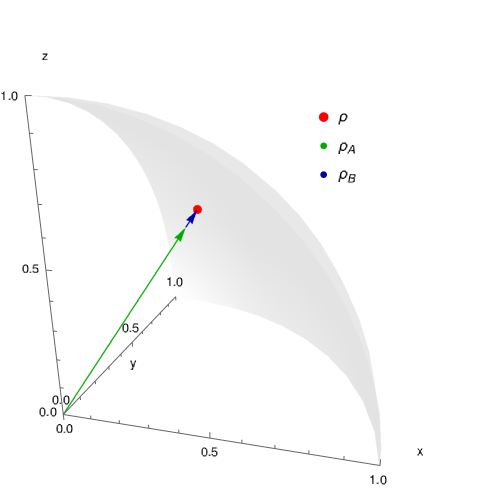
\includegraphics[width=0.75\columnwidth]{figures/effective_state_as_sum.png}%
                \caption{Effective state decomposed. $p=0.2$}
            \end{figure}
        \end{column}
    \end{columns}
\end{frame}

\begin{frame}{Quick review}
    \begin{displaymath}
        \xymatrix{
          {\rho(0)} \ar[rr]^{\Gamma_{t}} \ar[d]^{\mcA^{max}_{\mcC}}
          && {\rho(t)}\\
          {\varrho_{max}(0)} \ar[rr]^{\mcU_{t}}
          && {\varrho_{max}(t)} \ar[u]^{\mcC}
        }
      \end{displaymath}
      Where:
        \begin{equation*}
            \mcA_{\mcC}^{\max}[\rho]=\varrho_{max}=\rho_{A}\otimes\rho_{B} \qquad \mcU_{t}[\rho]=U^{t}\varrho(U^{t})^{\dag} \qquad \CG{\varrho}=\Tr_{2}((1-p)\varrho+pS\varrho S^{\dag})
        \end{equation*}
        \begin{equation*}
            \boxed{\Gamma_t[\rho]:=(\mcC \circ \mcU_t \circ \mcA^{max}_{\mcC})[\rho].}
        \end{equation*}
\end{frame}
\section{Effective dynamics}

\subsection{Separable dynamics}

\begin{frame}{General solution}
    Factorizable unitary dynamics are of the form $\mcU_{t}=U_{1}^{t}\otimes U_{2}^{t}$.
    \begin{align*}
        \text{Since } \varrho=\rho_{A}\otimes\rho_{B} & & \Longrightarrow & &\rho\mapsto pU_{1}^{t}\rho_{A}(U_{1}^{t})^{\dag}+(1-p)U_{2}^{t}\rho_{B} (U_{2}^{t})^{\dag}.
    \end{align*}
    Expected values evolve as
    \begin{align*}
        \begin{split}
            \expval{\pauli{i}(t)}=&\frac{p\tanh(p\lambda)}{2}\Tr[\pauli{i}U_{1}^{t}(\paulivec{r_{\rho}})(U_{1}^{t})^{\dag}]\\
        &+\frac{p\tanh((1-p)\lambda)}{2}\Tr[\pauli{i}U_{2}^{t}(\paulivec{r_{\rho}})(U_{2}^{t})^{\dag}].
        \end{split}
      \end{align*}
\end{frame}

\begin{frame}{Two cases}
    \begin{columns}
        \begin{column}{0.5\textwidth}
            \begin{itemize}
                \item Asume $U_{1}= U_{2}=U$.
                \item Thanks to symmetry, the evolution may be factored as
                \begin{align*}
                    \rho(t)&=pU^{t}\rho_{A}(U^{t})^{\dag}+(1-p)U^{t}\rho_{B}(U^{t})^{\dag} \\
                    &=U^{t}(p\rho_{A}+(1-p)\rho_{B})(U^{t})^{\dag}\\
                    &=U^{t}\rho(0)(U^{t})^{\dag}.
                    \end{align*}
                \item The effective dynamics are    
                \begin{equation*}
                    \rho\mapsto U^{t}\rho(U^{t})^{\dag}.
                \end{equation*}
            \end{itemize}
        \end{column}
        \begin{column}{0.5\textwidth}
            \begin{itemize}
                \item Asume either $U_{1}=\Id$ or $U_{2}=\Id$.
                \item Let $r_{A}\hat{r}_{\rho}$ and $r_{B}\hat{r}_{\rho}$ be the Bloch vectors of $\rho_{A}$ and $\rho_{B}$. Let $O_{i}$ be the rotation induced by $U_{i}$
                \item If $U_{2}=\Id$ then:
                \begin{equation*}
                    r\hat{r}_{\rho}\mapsto O_{1}(r\hat{r}_{\rho}-(1-p)r_{B}\hat{r}_{\rho})+(1-p)r_{B}\hat{r}_{\rho}.
                \end{equation*}
                \item If $U_{1}=\Id$ then:
                \begin{equation*}
                    r\hat{r}_{\rho}\mapsto r\hat{r}_{\rho}+(1-p)(O_{2}(r_{B}\hat{r}_{\rho})-r_{B}\hat{r}_{\rho}).
                \end{equation*}
            \end{itemize}
        \end{column}
    \end{columns}
\end{frame}




\begin{frame}{One example}
    \begin{columns}
        \begin{column}{0.5\textwidth}
            Let's consider an effective state
                \begin{equation*}
                    \rho=\frac{1}{2}(\Id+r_{z}\pauli{3}),
                \end{equation*}
            and an evolution $\mcU_{t}=e^{-itH_{1}}\otimes e^{-itH_{2}}$ where
                \begin{align*}
                    H_{1}=\pauli{3} & & \text{and} & & H_{2}=\frac{\omega}{\sqrt{2}}(\pauli{1}-\pauli{2}).
                \end{align*}
            We may solve this by using the formula
                \begin{equation*}
                    \rho\mapsto pU_{1}^{t}\rho_{A}(U_{1}^{t})^{\dag}+(1-p)U_{2}^{t}\rho_{B} (U_{2}^{t})^{\dag}.
                \end{equation*}
        \end{column}
        \begin{column}{0.5\textwidth}
            The unitaries might be written as
                \begin{equation*}
                    U_{1}^{t}=\Id\cos(\omega t) - i \pauli{3} \sin(\omega t),
                \end{equation*}
                \begin{equation*}
                    U_{2}^{t}=\Id\cos(\omega t) - \frac{i}{\sqrt{2}} (\pauli{1}-\pauli{2}) \sin(\omega t).
                \end{equation*}
                In a no-error scenario, we expect $\expval{\pauli{3}}=r_{z}$. Here, it is found to be:
                \begin{equation*}
                    \expval{\pauli{3}(t)}=\expval{\pauli{3}(0)}+(1-p)r_{B}(\cos(2\omega t)-1).
                \end{equation*}
            Note that $\expval{\pauli{3}(0)}$ is nothing but $r_{z}$.
        \end{column}
    \end{columns}
\end{frame}

\begin{frame}{Other states}
    \begin{columns}
        \begin{column}{0.5\textwidth}
            This oscillation is observable even if the initial efective state, $\rho$, is not invariant under the unitary $U_{1}$.
            
            Let $\rho$ be
            \begin{equation*}
                \rho=\frac{1}{2}\qty[\Id+\frac{4}{5\sqrt{2}}\qty(\frac{1}{2}\pauli{1}+\frac{1}{2}\pauli{2}+\pauli{3})]
            \end{equation*}
            Clearly, this state is not invariant under 
            \begin{equation*}
                U_{1}^{t}=\Id\cos(\omega t) - i \pauli{3} \sin(\omega t).
            \end{equation*}
        \end{column}
        \begin{column}{0.5\textwidth}
            \begin{figure}[h!]
                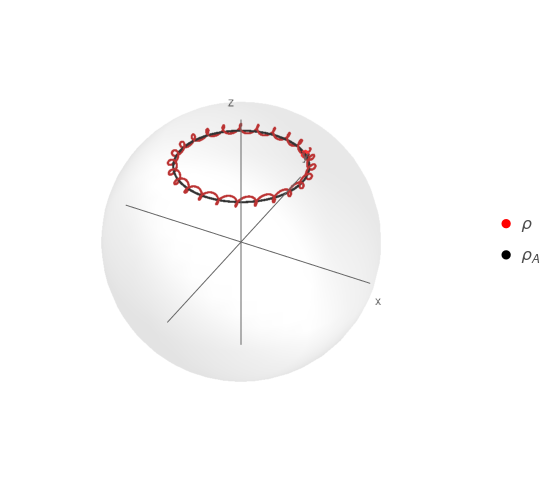
\includegraphics[width=0.8\columnwidth]{figures/U1xU2_H1=(sz)_H2=15(sx-sy)_z=0.8_p=0.9_wXY=0.5.png}%
                \caption{Small oscillations around the no-error trajectory. Here, $r=0.8$ $p=0.9$ and $\omega=15$. }
            \end{figure}
        \end{column}
    \end{columns}
\end{frame}



\subsection{Quantum computing gates}

\begin{frame}{Effective SWAP}
    State before and after the SWAP evolution is
    \begin{align*}
        \rho(0)&=\frac{1}{2}[\Id+(\hat{r}_{\rho}\cdot\vec{\sigma})(p\tanh{-\lambda p}+(1-p)\tanh{-\lambda (1-p)})],\\
        \rho(t=1)&=\frac{1}{2}[\Id+(\hat{r}_{\rho}\cdot\vec{\sigma})((1-p)\tanh{-\lambda p}+p\tanh{-\lambda (1-p)})].
        \end{align*}
    Both states have the same orientation, but different purity. The effective dynamics are described by a contraction of the Bloch sphere. Contraction factor depends on $\lambda(\rho)$:
    \begin{equation*}
        \kappa_{1}=\frac{r_{\rho(1)}}{r_{\rho(0)}}=\frac{(1-p)\tanh{\lambda p}+p\tanh{\lambda (1-p)}}{
          p\tanh{\lambda p}+(1-p)\tanh{\lambda (1-p)}}.
      \end{equation*}
      This evolution can be written as
      \begin{equation*}
        \boxed{\frac{1}{2}(\Id+\vec{r}_{\rho}\cdot\vec{\sigma}) \xrightarrow{S} \frac{1}{2}(\Id+\kappa_{1}^{\rho}\vec{r}_{\rho}\cdot\vec{\sigma})}
      \end{equation*}
\end{frame}

\begin{frame}{The contraction factor}
    \begin{figure}[h!]
        \centering
        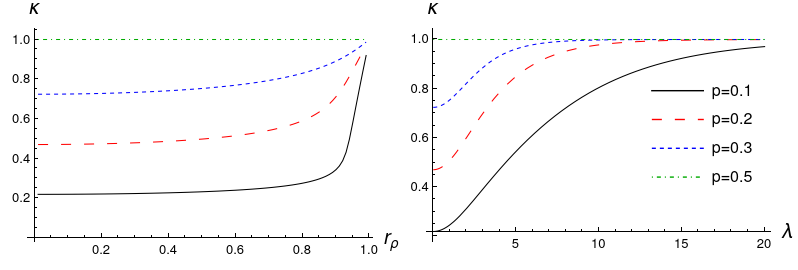
\includegraphics[width=0.9\linewidth]{figures/ContractionFactorSWAP_2D_both.png}
        \caption{$\kappa_{1}$ as a function of the initial purity $r_{\rho}$ (left) and as a function of the Lagrange multipliers $\lambda$ (right), for different values of $p$.}
        \label{fig:SWAPFactor2D}
      \end{figure}
\end{frame}

\begin{frame}{Generalized SWAP gate}
    SWAP gate might be extended to an arbitrary time as $S^{t}$. In this case, 
    \begin{equation*}
        \kappa_{t}^{\rho}=\frac{((1-p)\cos^{2}{\frac{\pi t}{2}}+p\sin^{2}{\frac{\pi t}{2}})\tanh{\lambda p}+(p\cos^{2}{\frac{\pi t}{2}}+(1-p)\sin^{2}{\frac{\pi t}{2}})\tanh{\lambda (1-p)}}{
          p\tanh{\lambda p}+(1-p)\tanh{\lambda (1-p)}}.
      \end{equation*}
      In terms of the spin observable $\sigma_{z}$, evolution looks like
\begin{equation}
  \expval{\sigma_{z}(t)}=\kappa_{t}^{\rho}\expval{\sigma_{z}(0)}.
\end{equation}
Or, in terms of the probability of getting either $\ket{0}$ or $\ket{1}$ as
 \begin{align}
  \bra{0}\rho(t)\ket{0}=\frac{1}{2}(1+\kappa_{t}^{\rho}\expval{\sigma_{z}(0)}) && \bra{1}\rho(t)\ket{1}=\frac{1}{2}(1-\kappa_{t}^{\rho}\expval{\sigma_{z}(0)}),
 \end{align}
 where both non linearity and time dependency is contained inside the contraction factor $\kappa_{t}^{\rho}$. 
\end{frame}

\begin{frame}{Periodicity of the effective SWAP gate}
    \begin{figure}[h!]
        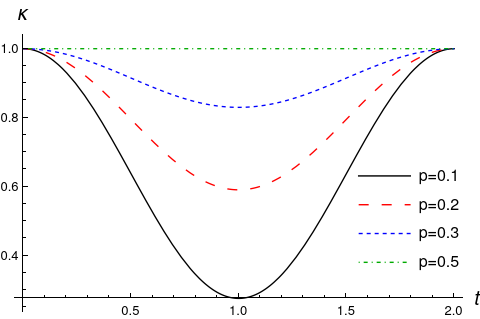
\includegraphics[width=0.5\columnwidth]{figures/ContractionFactorSWAP_z=0.8_t=0_to_t=2.png}%
        \caption{The contraction factor as a function of $t$, for different values of $p$ and $r=0.8$. Note the periodic nature of the effective evolution.}
    \end{figure}
\end{frame}

\begin{frame}{Effect on the Bloch sphere}
    \begin{figure}[h!]
        \centering
        \begin{subfigure}{0.32\textwidth}
            \centering
            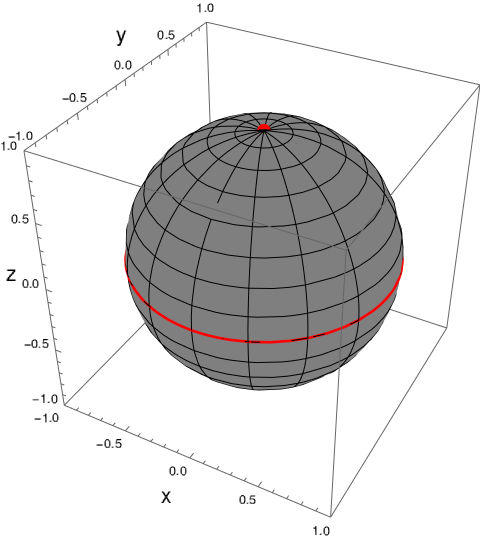
\includegraphics[width=0.9\linewidth]{figures/sphere_swapcontraction_t=0.0_z=0.9_p=0.9.png}
            \caption{$t=0.0$}
        \end{subfigure}%
        \begin{subfigure}{0.32\textwidth}
            \centering
            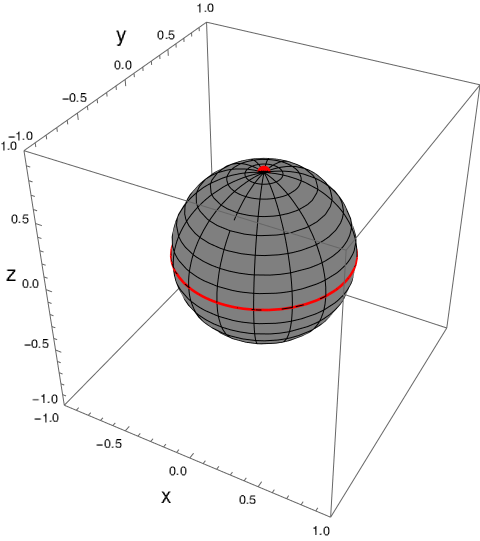
\includegraphics[width=0.9\linewidth]{figures/sphere_swapcontraction_t=0.5_z=0.9_p=0.9.png}
            \caption{$t=0.5$}
        \end{subfigure}
        \begin{subfigure}{0.32\textwidth}
            \centering
            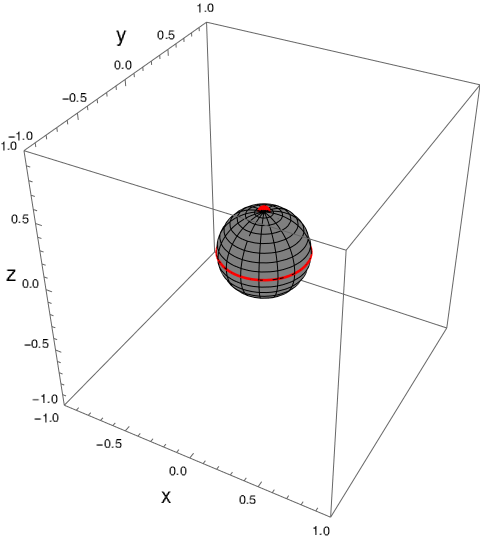
\includegraphics[width=0.9\linewidth]{figures/sphere_swapcontraction_t=1.0_z=0.9_p=0.9.png}
            \caption{$t=1.$}
        \end{subfigure}
        \caption{Effect on the Bloch sphere. $r=0.9$, $p=0.9$. The dramatic contraction can be associated with the near total loss of information.}
    \end{figure}
\end{frame}
\begin{frame}{Periodicity of the effective SWAP gate}
    \begin{figure}[h!]
        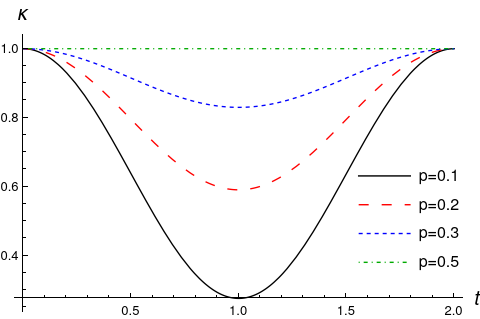
\includegraphics[width=0.5\columnwidth]{figures/ContractionFactorSWAP_z=0.8_t=0_to_t=2.png}%
        \caption{The contraction factor as a function of $t$, for different values of $p$ and $r=0.8$. Note the periodic nature of the effective evolution.}
    \end{figure}
\end{frame}



\begin{frame}{CNOT gate}
    The controlled not gatis generated by a hamiltonian
    \begin{equation*}
        H_{\cnot}=\frac{\pi}{4}\qty(\Id-\pauli{3}\otimes\Id-\Id\otimes\pauli{1}+\pauli{3}\otimes\pauli{1}),
    \end{equation*}
    From this, it is possible to expand the gate as three succesive unitary operators
    \begin{align*}
        \cnot&=e^{-i\frac{\pi}{4}\Id}e^{i\frac{\pi}{4}\pauli{3}\otimes\Id}e^{i\frac{\pi}{4}\Id\otimes\pauli{1}}e^{-i\frac{\pi}{4}\pauli{3}\otimes\pauli{1}}\\
        &=e^{-i\frac{\pi}{4}} (e^{i\frac{\pi}{4}\pauli{3}}\otimes \Id) (\Id \otimes e^{i\frac{\pi}{4}\pauli{1}}) e^{-i\frac{\pi}{4}\pauli{3}\otimes\pauli{1}}.
    \end{align*}
    While the usual CNOT interpretation of the gate might be blurry, another one arises: the CNOT gate induces correlations between the $\pauli{3}$ component of the first subsystem and the $\pauli{1}$ component of the second subsystem.
\end{frame}

\begin{frame}{Effective CNOT}
    Let's suppose for a moment than $p=1$. The evolved effective state will be
    \begin{equation*}
      \rho(t=1)=\rho(0)+\pauli{3}\rho(0)\pauli{3}=\frac{1}{2}(\Id+r_{3}\pauli{3}).
    \end{equation*}
    This is because the MaxEnt state will be $\rho\otimes\frac{1}{2}$. The $\pauli{1}$ and $\pauli{2}$ components are lost because the CNOT gate applies a $\pauli{3}$ gate on the first particle depending on the value of the second particle in the $\pauli{1}$ basis. If the second particicle finds itself on the state $\frac{1}{2}\Id$, the \textit{application rate} of the $\pauli{3}$ gate (that changes the $\pauli{1}$ and $\pauli{3}$ components) will be equally random: the information is lost.
\end{frame}

\begin{frame}{Effective CNOT}
    State before and after the CNOT evolution is
    \begin{align*}
        \rho(0)=&\frac{1}{2}[\Id+(\hat{r}_{\rho}\cdot\vec{\sigma})(p\tanh{-\lambda p}+(1-p)\tanh{-\lambda (1-p)})],\\
        \rho(t=1)=&\frac{1}{2}[p(\rho(0)+\sigma_{3}\rho_{A}\sigma_{3}+\Tr{\sigma_{1}\rho_{B}}[\rho_{A}-\sigma_{3}\rho_{A}\sigma_{3}])\\
    &+(1-p)(\rho(0)+\sigma_{1}\rho_{B}\sigma_{1}+\Tr{\sigma_{3}\rho_{A}}[\rho_{B}-\sigma_{1}\rho_{B}\sigma_{1}])].
        \end{align*}
    Notice the similarity between this expression and the previous one. The CNOT gate induces correlations between both subsystems. These corrleations are completely dependent on the $\pauli{3}$ and $\pauli{1}$ components of the first and second subsystem.
    The second term shows the action of the \textit{target} qubit over the \textit{control} qubit on the $\pauli{1}$ basis.
\end{frame}

\begin{frame}{Effective CNOT on the Bloch sphere}
    \begin{figure}[h!]
        \centering
        \begin{subfigure}{0.32\textwidth}
            \centering
            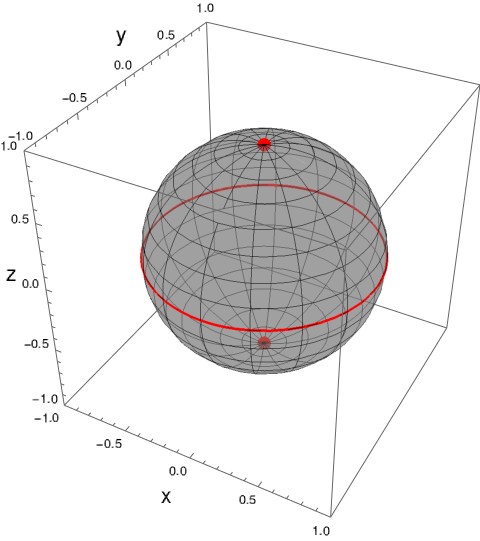
\includegraphics[width=0.9\linewidth]{figures/sphere_CNOT_t=0.0_z=0.8_p=0.95.png}
            \caption{$t=0.0$}
        \end{subfigure}%
        \begin{subfigure}{0.32\textwidth}
            \centering
            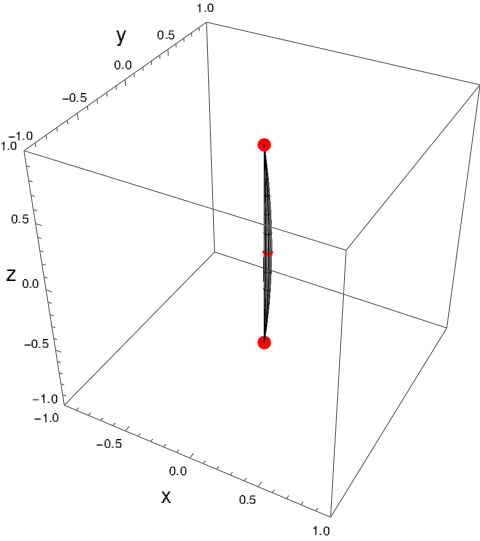
\includegraphics[width=0.9\linewidth]{figures/sphere_CNOT_t=1.0_z=0.8_p=0.95.png}
            \caption{$t=0.5$}
        \end{subfigure}
        \caption{Effect on the Bloch sphere. $r=0.8$, $p=0.95$.}
    \end{figure}
\end{frame}

\begin{frame}{Effective CNOT on the Bloch sphere}
    \begin{figure}[h!]
        \centering
        \begin{subfigure}{0.32\textwidth}
            \centering
            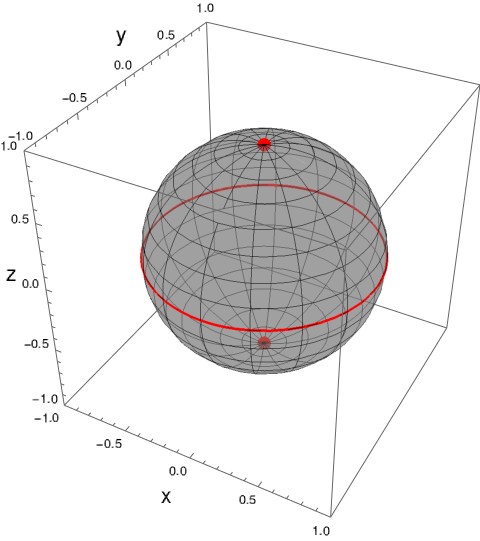
\includegraphics[width=0.9\linewidth]{figures/sphere_CNOT_t=0.0_z=0.8_p=0.6.png}
            \caption{$t=0.0$}
        \end{subfigure}%
        \begin{subfigure}{0.32\textwidth}
            \centering
            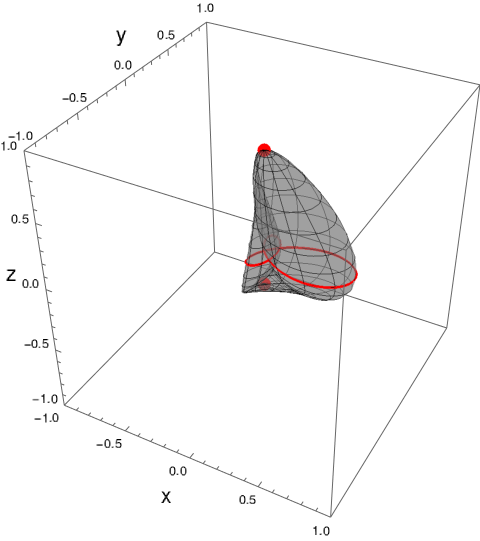
\includegraphics[width=0.9\linewidth]{figures/sphere_CNOT_t=1.0_z=0.8_p=0.6.png}
            \caption{$t=0.5$}
        \end{subfigure}
        \caption{Effect on the Bloch sphere. $r=0.8$, $p=0.6$.}
    \end{figure}
\end{frame}

\subsection{Special Dynamics}

\begin{frame}{Ising Model}
    We consider the following hamiltonian:
    \begin{align*}
        H=J\sigma_{z}\otimes\sigma_{z} && \Rightarrow && \mcU_{t}=\Id \cos{tJ} + i\sigma_{z}\otimes\sigma_{z}\sin{tJ}
    \end{align*}
    The evolved effective state looks like
    \begin{align*}
        \mcC{\varrho_{max}(t)}=&\rho(0)\cos^{2}{Jt}+\sigma_{3}\rho(0)\sigma_{3}\sin^{2}{Jt}\\
        &-i\frac{\lambda_{3}}{\lambda}\sin{Jt}\cos{Jt}[\sigma_{3},p\tanh((1-p)\lambda)\rho_{A}+(1-p)\tanh(p\lambda)\rho_{B}]
    \end{align*}
    Two important terms arise: the first is linear and independent of the coarse graining parameters, and the second one carries the non-linearity of the evolution, as it includes the Lagrange variable $\lambda$.
\end{frame}
\chapter{Conclusiones}

\ddnote{Comienza explicando que hiciste. Tipo: se estudió la dinámica emergente al combinar el principio de MaxEnt con un modelo de grano grueso, tal que en el nivel fino se cumple la mecánica cuántica. En particular se estudiaron los sistemas tales, presentados en el capitulo tal.}


\ddnote*{ideas buenas, pero muy cantinfleado, el párrafo es una sola frase también :S. No hay necesidad de ser extremadamente breves, explica con calma y separando en más oraciones}{Se estudió la dinámica efectiva que emergió de considerar un modelo de grano grueso que relaciona un estado efectivo de un qubit a un espacio microscópico de $n$ qubits, de utilizar el Principio de Máxima Entropía para hallar un estado fino compatible con dicho estado efectivo, y de asumir que el sistema microscópico evoluciona de acuerdo a las leyes de la mecánica cuántica.}

Se introdujo una aplicación de grano grueso que modela dos tipos de errores. El primero es el inducido por un aparato que tiene una probabilidad no nula de medir una partícula diferente a la pretendida. El segundo proviene de la incapacidad del detector de resolver todos los grados de libertad del sistema. Esta falta de resolución provoca que el sistema de $n$ qubits se vea como un sistema de uno solo. Se construyó una aplicación de asignación basada en el Principio de Máxima Entropía para hallar al estado microscópico menos sesgado posible, tal que fuera compatible con un estado efectivo dado. Asumiendo que el sistema fino evoluciona de manera que cumple con las leyes de la mecánica cuántica, se estudiaron las dinámicas efectivas inducidas por dichas evoluciones, el modelo de grano grueso y la aplicación de asignación.

\acnote{Arranca mejor la primera versión. La primera frase de un párrafo debe explicar el contenido del párrafo. El modelo de grano grueso no modela dos tipos de errores. El modelo de grano grueso surge de la concatenación de dos tipos de errores.}

Como se discutió en el capítulo \ref{sec:chapter2}, del modelo de grano grueso utilizado se reconocieron dos regímenes particularmente interesantes, \acnote{régimen imparical} \ddnote*{discutamos este nombre. Propongo algo como \textit{caso no sesgado}}{el régimen de Boltzmann}, asociado a una caja de $n$ partículas idénticas en la que cada una es igualmente probable de ser medida, y el régimen de partícula preferencial, en el que una partícula tiene una probabilidad mucho mayor de ser medida. En estos regímenes, la asignación de máxima entropía está dada por las ecuaciones (\ref{eq:BoltzmannAss}) y (\ref{eq:PreferentialAss}) respectivamente.

\ddnote*{De acuerdo a lo hallado en el capítulo \ref{sec:chapter3}, a través de la utilización de un modelo de grano grueso para estudiar la dinámica efectiva de sistemas de muchas partículas (ver ecuación tal (esas donde muestras la concatenación)), es posible hallar comportamientos más afines a la física clásica que a la mecánica cuántica, como la no linealidad de las evoluciones.}{De acuerdo a lo hallado en el capítulo \ref{sec:chapter3}, a través de la utilización de un modelo de grano grueso para estudiar la dinámica efectiva de sistemas de muchas partículas es posible hallar comportamientos más afines a la física clásica que a la mecánica cuántica, como la no linealidad de las evoluciones.} Sin embargo, las no linealidades encontradas, a diferencia de las dinámicas clásicas no lineales, no son universales. Esto debido a que todas resultaron dependientes del estado efectivo inicial. 
%
Otra diferencia viene del hecho que las evoluciones clásicas \ddnote{$deterministas$} no conllevan cambios en la entropía del sistema, mientras que las evoluciones efectivas estudiadas se traducían en contracciones de la esfera de Bloch, quizá mejor representadas por la compuerta SWAP efectiva, (\ref{eq:EffectiveSWAPt}). Dicho de otra forma, las dinámicas efectivas resultaron ser procesos irreversibles \ddnote*{, manifestado en el aumento de la entropía del sistema.}{con cambios en la entropía del sistema efectivo.}

Alguna de las dinámicas estudiadas, particularmente aquellas generadas por evoluciones subyacentes con fuertes simetrías, resultaron ser no solo lineales, sino canales cuánticos, como el caso de ciertos tipos de canales de Pauli, (\ref{eq:EffectiveDephasing}) y (\ref{eq:EffectiveDepolarizing}), y el canal de estabilización (\ref{eq:EffectiveStabilizing}), o aún más, evoluciones unitarias, como el caso de la dinámica local simétrica (\ref{eq:EffectiveSymmetricLocal}). 

Ninguna de las dinámicas estudiadas es no lineal en el caso en que las partículas no preferenciales tienen una probabilidad nula de ser detectadas, esto es, cuando el error es nulo, que equivale al caso en que la aplicación de medición borrosa sale del escenario. Aunque el único elemento no lineal en la composición que define a la dinámica efectiva es la aplicación de asignación, queda por investigar si es la aplicación de asignación o la aplicación de medición borrosa la causante de las no linealidades en las dinámicas efectivas.
\ddnote{Mañana hagamos un recuento de observaciones, para ver que mas ponemos aquí.}


\appendix

\begin{frame}{References}
\begin{thebibliography}{99}
\bibitem ONielsen, M. \& Chuang, L. (2010).\textit{Quantum Computation and Quantum Information}. Cambridge, United Kingdom: Cambridge University Press.
\bibitem OSilva, P. \& Concha, P. \& Vallejos, R. \& de Melo, F. (2020).\textit{Macro-to-micro quantum mapping and the emergence of nonlinearity}. PsyArXiv. DOI:10.1103/PhysRevA.103.052210
\end{thebibliography}
\end{frame}

\section{Appendix}

\begin{frame}{A1. Lagrange \textit{variable} and purity}
    \begin{columns}
        \begin{column}{0.5\textwidth}
            Having $\varrho_{max}$ in terms of $\lambda$ instead of observables is not ideal. The effective state is
            \begin{equation*}
                \rho=\frac{1}{2}(\Id+r_{\rho}\hat{r}_{\rho}\cdot\vec{\sigma}).
            \end{equation*}
            The relation between the observables and the Lagrange variable is
            \begin{equation*}
                r_{\rho}=(1-p)\tanh{\lambda (1-p)}+p\tanh{\lambda p}.
            \end{equation*}
        \end{column}
        \begin{column}{0.5\textwidth}
            \begin{figure}[h!]
                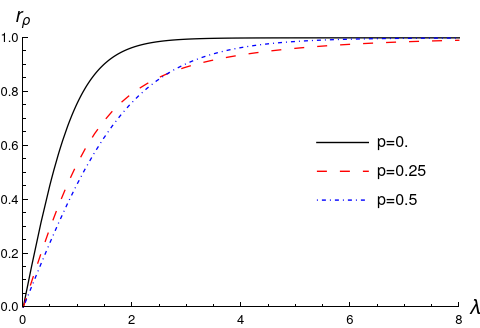
\includegraphics[width=0.8\columnwidth]{figures/r(lambda).png}%
                \caption{$r_{\rho}$ as a function of $\lambda$ for different values of $p$}
            \end{figure}
        \end{column}
    \end{columns}
\end{frame}


\end{document}
